\newcommand\ddiff[1]{\ddot{#1}}
\newcommand\diff[1]{\dot{#1}}

\subsection{ Geodæt på ``æggebakke'' }
Vi vil i dette afsnit forsøge at finde geodæter på en ``æggebakke'',
en flade givet ved:
\begin{equation}\label{eq:aeggebakke}
F(x,~y) = (x,~y,~a \cdot \cos(x)+~a \cdot \sin(y))
\end{equation}
Variablen \(a\) bestemmer ``dybden'' på æggebakken.
Grafen for en æggebakke med \(a = 2\) er plottet i figur~\ref(fig:aeg)
\begin{figure}[h!]
  \centering
    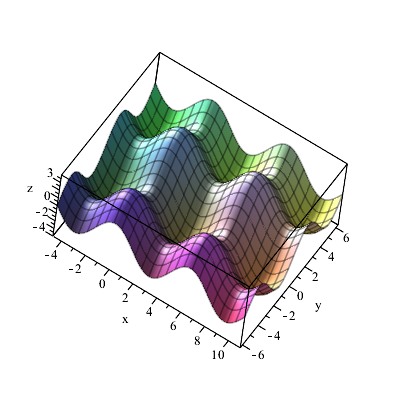
\includegraphics[width=0.5\textwidth]{aeg}
    \caption{Plot af fladen \(F(x,~y) = (x,~y,~a \cdot \cos(x)+~a \cdot \sin(y))\) for \(a=2\)}\label{fig:aeg}
\end{figure}
Det vil dog vise sig at dette ikke altid er ligetil at finde geodæter på flader af denne type.

\subsubsection{Geodæter på flader af typen \(\mathscr{F}(x,~y) = (x,~y,~f(x,~y))\)}
Lad os først se, hvad der kræves for at finde geodæter på flader af typen:
\begin{equation*}
\mathscr{F}(x,~y) = (x,~y,~f(x,~y))
\end{equation*}

med geodæter af typen:
\begin{equation} \label{eq:geodPlanFlade}
\pmb{\gamma}(t) = (x(t),~y(t),~f(x(t),~y(t)))
\end{equation}

%Jf. noget david har skrevet, for håbentligt! Ellers får jeg travlt
har vi følgende Euler-Lagrange ligninger:
\begin{equation*}
\begin{gathered}
\frac{\partial L}{\partial x} - \frac{d}{dt}\frac{\partial L}{\partial \diff{x}} = 0\\
\frac{\partial L}{\partial y} - \frac{d}{dt}\frac{\partial L}{\partial \diff{y}} = 0
\end{gathered}
\end{equation*}

\paragraph{Geodæt på flat plan}
Lad os se hvad dette gør for geodæter på det simple plan:
\begin{equation}\label{eq:P}
P(x,~y) = (x,~y,~k)
\end{equation}
da vi ved at disse bliver til rette linjer (det svarer til at finde geodæter i \(\mathbb{R}\))
%
Vi får da en geodæt på formen:
\begin{equation*}
\pmb{\gamma_p}(t) = (x(t),~y(t),~k)
\end{equation*}
%
og Lagrange funktionen:
\begin{equation*}
L(\pmb{\gamma_p}) = \sqrt{ \diff{x}(t)^2 + \diff{y}(t)^2 }
\end{equation*}
%
hvilket giver følgende Euler-Lagrange ligninger:
\begin{equation} \label{eq:ELPlanFlade}
\begin{gathered}
\frac{\partial L}{\partial x} - \frac{d}{d t} \frac{\partial L}{\partial \diff{x}} =
\frac{\diff{y}(t) \cdot ( \ddiff{x}(t)\diff{y}(t) - \ddiff{y}(t)\diff{x}(t) )}{\sqrt{\diff{x}(t)^2 + \diff{y}(t)^2}^3} = 0\\
\frac{\partial L}{\partial y} - \frac{d}{d t} \frac{\partial L}{\partial \diff{y}} =
\frac{\diff{x}(t) \cdot ( \ddiff{x}(t)\diff{y}(t) - \ddiff{y}(t)\diff{x}(t) )}{\sqrt{\diff{x}(t)^2 + \diff{y}(t)^2}^3} = 0\\
\end{gathered}
\end{equation}
%
dette betyder at hverken  \( \diff{x}(t) \) eller \(\diff{y}(t) \) må være nulfunktionen,
da dette ville resultere i at nævneren også bliver nul.

Den nemme løsning ville være at sætte \(\ddiff{x}(t)\) og \(\ddiff{y}(t)\) til at være nulfunktionerne,
hvilket naturligvis ville resultere i en ret linje med ligningen:
\begin{equation*}
\pmb{p_1}(t) = (C_1 + C_2\cdot t,~C_2 + C_3\cdot t,~k)
\end{equation*}

Men dette er ikke den eneste løsning. Det skarpe øje vil skue, at hvis
\( \ddiff{x}(t)\diff{y}(t) = \ddiff{y}(t)\diff{x}(t) \)
bliver tælleren også \(0\), en anden simpel løsning på ligningssystemet er da:
\begin{equation*}
\pmb{p_2}(t) = (C_1 + C_2\cdot m(t),~C_2 + C_3\cdot m(t),~k)
\end{equation*}
da
\begin{equation*}
\begin{gathered}
\frac{d^2}{dt^2} (C_1 + C_2\cdot m(t)) \frac{d}{dt} (C_3 + C_4\cdot m(t)) = C_2\ddiff{m}(t) C_4\diff{m}(t) \\
 = \frac{d}{dt} (C_1 + C_2\cdot m(t)) \frac{d^2}{dt^2} (C_3 + C_4\cdot m(t)) = C_2\diff{m}(t) C_4\ddiff{m}(t) 
\end{gathered}
\end{equation*}
dette kræver selvfælgelig at \( m(t) \) er monoton og differentiabel to gange i det interval, \(t\) løber over.
Ellers kan differentialligningen ikke tilfredsstilles.

De to funktioner \(\pmb{p_1}(t)\) og \(\pmb{p_2}(t)\) har naturligvis samme kurve,
ellers var de jo ikke begge geodæter til samme flade, den eneste forskel er at \(t\) ``løber'' med forskellig hastighed.
Da vi kan lade parameteren for en hver funktion løbe efter \(m(t)\), uden at kurven for denne ændre længde,
betyder det at alle geodæter på formen (\ref{eq:geodPlanFlade}) vil have arbitrære ligninger i deres løsning.
%For overfladisk?

Der skal dog ikke meget til at forestille sig en flade med en Euler-Lagrange ligning, der er så kompliceret,
at denne ikke kan løses ved simple ``tricks''. Ønsker man i midlertid at tage \emph{CAS}-programmet \emph{Maple}
i brug, vil dette også volde en problemer,
da det ikke er muligt for \emph{Maple} at løse differential-ligninger med arbitrære funktioner i løsningen.

Derfor er det nødvendigt at parametriserer geodæten yderligere. Hvis vi vælger en parametrisering så
\begin{gather*}
x(t) = p(t,~m(t))\\
y(t) = q(t,~m(t))
\end{gather*}
hvor et valg af \(p\) og \(q\) definerer parametriserinen og \(m(t)\) er ligningen, der løses efter.
Dette kræver dog at der findes geodæter af denne type.

Lad os igen kigge på geodæten \(\pmb{\gamma_p}\) og se hvad der sker,
hvis vi parametriserer denne,
så \(p(t,~m(t) ) = t\) og \(q(t,~m(t) ) = m(t)\).
Vi får da en geodæt på formen:
\begin{equation*}
\pmb{\gamma_p}(t) = (t,~m(t),~k)
\end{equation*}
%
og Lagrange funktionen:
\begin{equation*}
L(\pmb{\gamma_p}) = \sqrt{ 1 + \diff{m}(t)^2 }
\end{equation*}

Vi ser at Lagrange funktionen her er afhænging af \(\diff{m}(t)\) 
hvilket giver følgende Euler-Lagrange ligning:
\begin{equation*}
\frac{\partial L}{\partial m} - \frac{d}{d t} \frac{\partial L}{\partial \diff{m}} = 
\frac{\ddiff{m}(t)}{\sqrt{1 + \diff{m}(t)^2}^3} = 0\\
\end{equation*}

Det er her tydeligt at se, at løsningen er givet, når \(\ddiff{m}(t) = 0\)

Denne ligning giver én entyding løsning, uden arbitrære funktioner:
\begin{equation*}
m(t) = C_1 + C_2 \cdot t
\end{equation*}

Dette giver geodæter af typen:
\begin{equation*}
\pmb{\gamma_p}(t) = (t,~C_1 + C_2 \cdot t,~k)
\end{equation*}
 
 Ønsker vi at finde geodæten mellem to punkter, skal vi blot løse en ligning med hensyn til \(C_1\) og \(C_2\)
 Der er dog det problem, at ikke alle geodæter til (\ref{eq:P}) er af denne type.
 Geodæten fra \((0,~0)\) til \((0,~1)\) er for eksempel ikke af denne type, da dette giver
 \begin{equation*}
 \pmb{\gamma_p}(0) = (0,~0,~k) \neq  \pmb{\gamma_p}(0) = (0,~1,~k)
 \end{equation*}

Konklutionen er at det ofte simplifiserer differentialligingerne,
at parametriserer geodæter af typen (\ref{eq:geodPlanFlade}) til
\begin{equation*}
\pmb{\gamma}(t) = (p(t,~m(t)),q(t,~m(t)),~f(x(t),~y(t)))
\end{equation*}
blot skal man være opmærksom på at vælge en parametrisering, der ikke udelukker den geodæt der ledes efter.

\subsubsection{Geodæt for æggebakke }

Vi kan nu begynde at finde geodæter på flader, formet ``som æggebakker''.

Først findes Euler-Lagrange ligninger for geodæter af typen:
\begin{equation}\label{eq:aeggegeo}
\pmb{\gamma}(t) = (x(t),~y(t),~a\cos(x(t)) + a\sin(y(t)))
\end{equation}

Lagrange funktionen findes nemt:
\begin{equation*}
L(\pmb{\gamma}(t)) = \sqrt{\diff{x}(t)^2 + \diff{y}(t)^2 + ( -a \cdot \sin(x(t)) + a \cdot \cos(y(t)) )^2}
\end{equation*}
 
\begin{lstlisting}[caption=Udregning af de to Lagrange ligninger til (\ref{eq:aeggegeo}) med \emph{Maple}  ]
>F:=(x,y) -> <x, y, a*cos(x) + a*sin(y)>:

>L:=sqrt( diff(F(x(t),y(t))[1],t)^2 + diff(F(x(t),y(t))[2],t)^2 +diff(F(x(t),y(t))[3],t)^2 ):
>L:= subs(diff('x(t)',t)=dx, diff('y(t)',t)=dy, 'x(t)'=x1, 'y(t)'=y1, L):

>dLdy := diff(L,y1):
>dLddy := diff(L,dy):
>dLdx := diff(L,x1):
>dLddx := diff(L,dx):

>dLdx := subs(dx=diff(x(t),t), dy=diff(y(t),t), x1=x(t), y1=y(t), dLdx):
>dLddx := subs(dx=diff(x(t),t), dy=diff(y(t),t), x1=x(t), y1=y(t), dLddx):
>dLdy := subs(dx=diff(x(t),t), dy=diff(y(t),t), x1=x(t), y1=y(t), dLdy):
>dLddy := subs(dx=diff(x(t),t), dy=diff(y(t),t), x1=x(t), y1=y(t), dLddy):

>diflx := simplify(dLdx - diff(dLddx,t)) = 0;
>difly := simplify(dLdy - diff(dLddy,t)) = 0;
\end{lstlisting}

I linje 4 foretages et antal erstatninger,
der tillader \emph{Maple} at differenterer med hensyn til en funktion og dens afledte.
I linerne 6-9 udregnes \(\frac{\partial L}{\partial x}\), \(\frac{\partial L}{\partial y}\),
 \(\frac{\partial L}{\partial \diff{x}}\) og \(\frac{\partial L}{\partial \diff{y}}\).
I linjerne 11-14 substitueres modsat af lineje 4, så \(dx\) bilver til \(\diff{x}(t)\) etc.
I linje 16 og 17 udregnes og simplifiseres Euler-Lagragne lingningerne.
Ligningene givet fra \emph{Maple} er
\begin{multline*}
\frac{\partial L}{\partial x} - \frac{d}{d t} \frac{\partial L}{\partial \diff{x}} = 
\Big(
\diff{y}(t)(-a^2\sin(x(t))\sin(y(t))\diff{y}(t)^3)
- \ddiff{x}(t) a^2 \cos(y(t))^2 \diff{y}(t) - a^2\ddiff{x}\diff{y}(t)\\
+ a^2\ddiff{x}(t)\diff{y}(t)\cos(x(t))^2 - \diff{x}(t)a^2\ddiff{y}(t)\cos(x(t))^2
+ \diff{x}(t) \ddiff{y}(t) + \diff{x}(t)a^2\ddiff{y}(t)
\Big) \left. \middle/ \phantom{\Big(} \right.\\
\Big( \diff{x}(t)^2 + \diff{y}(t)^2 + a^2\diff{x}(t)^2 - a^2\diff{x}(t)^2\cos(x(t))^2\\
 - 2a^2\sin(x(t))\diff{x}(t)\cos(y(t))\diff{y}(t) + a^2 \cos(y(t))^2\diff{y}(t)^2 \Big)^{3/2} = 0
\end{multline*}
og
\begin{multline*}
\frac{\partial L}{\partial y} - \frac{d}{d t} \frac{\partial L}{\partial \diff{y}} = 
\Big(
\diff{x}(t)(-a^2\sin(x(t))\sin(y(t))\diff{y}(t)^3)
- \ddiff{x}(t) a^2 \cos(y(t))^2 \diff{y}(t) - a^2\ddiff{x}\diff{y}(t)\\
+ a^2\ddiff{x}(t)\diff{y}(t)\cos(x(t))^2 - \diff{x}(t)a^2\ddiff{y}(t)\cos(x(t))^2
+ \diff{x}(t) \ddiff{y}(t) + \diff{x}(t)a^2\ddiff{y}(t)
\Big) \left. \middle/ \phantom{\Big(} \right.\\
\Big( \diff{x}(t)^2 + \diff{y}(t)^2 + a^2\diff{x}(t)^2 - a^2\diff{x}(t)^2\cos(x(t))^2\\
 - 2a^2\sin(x(t))\diff{x}(t)\cos(y(t))\diff{y}(t) + a^2 \cos(y(t))^2\diff{y}(t)^2 \Big)^{3/2} = 0
\end{multline*}
Dette er en koblet, ulineær differentialligning af \(2.\) orden.
Ummidelbart er der ingen nemme løsninger, som i (\ref{eq:ELPlanFlade}).
\emph{Maple} kan heller ikke hjælpe os, hvilket ikke kommer som en overraskelse.

\paragraph{Parametrisering af geodæt for æggebakke}
Vi kan vælge en parametrisering så:
\begin{equation}\label{eq:aeggegeonem}
\pmb{\gamma}(t) = ( t ,~m(t),~a\cos(t) + a\sin(m(t)))
\end{equation}
Dette begrænser naturligvis de geodæter vi kan finde, men det simplificerer problemet betydeligt.

\begin{lstlisting}[caption=Udregning af de to Lagrange ligninger til (\ref{eq:aeggegeonem}) med \emph{Maple}  ]
F:=(x,y) -> <x, y, a*cos(x) + a*sin(y)>:
x:=t -> t:
y:=t -> m(t):
L:=sqrt( diff(F(x(t),y(t))[1],t)^2 + diff(F(x(t),y(t))[2],t)^2 +diff(F(x(t),y(t))[3],t)^2 );

L:= subs( diff('m(t)',t)=dm, 'm(t)'=m1, L ):
dLdm := subs( dm=diff(m(t),t), m1=m(t), dLdm):
dLddm := subs( dm=diff(m(t),t), m1=m(t), dLddm):

diflm := simplify(dLdm - diff(dLddm,t)) = 0;
\end{lstlisting}

Dette giver Lagrange ligningen
\begin{equation*}
L(\pmb{\gamma}(t)) = \sqrt{ 1 + \diff{m}(t)^2 + ( -a\sin(t) + a\cos(m(t))\diff{m}(t)}
\end{equation*}
og Euler-Lagrange ligningen:
\begin{multline*}
\frac{\partial L}{\partial m} - \frac{d}{d t} \frac{\partial L}{\partial \diff{m}} = 
\Big( a^2\cos(m(t))sin(m(t))\diff{m}(t)^2 + \diff{m}(t)a^2\sin(t)\cos(t)
+ a^2\sin(t)\sin(m(t))\diff{m}(t)^3\\
- \ddiff{m}(t) - \ddiff{m}(t)a^2
+ \ddiff{m}(t) a^2 \cos(t)^2 + a^2\cos(m(t))\cos(t) - a^2\cos(m(t))^2\ddiff{m}(t)
\left.\Big)\middle/\right.\\
\Big(
1 + \diff{m}(t)^2 + a^2 - a^2\cos(t)^2 - 2 a^2\sin(t)cos(m(t))\diff{m}(t)
+a^2\cos(m(t))^2\diff{m}(t)^2
\Big)^{3/2} = 0
\end{multline*}

Dette er stadig en ulineær differentiallilgnign af \(2.\) grad, men nu har \emph{Maple} en mulighed for at løse den,
til dette benytte \emph{dsolve}. Dette er dog kun muligt for \emph{Maple} at løse denne, når dette gøres nummerisk.

Følgensde betingelser vælges for \(m(t)\):
\begin{align*}
m(-\pi) &= 1\\
m(3\pi) &= 1\\
\end{align*}

Desuden skal der vælges en værdi for \(a\).
For at vise hvordan geodæten ændre sig i takt med at \(a\) ændre sig,
løses problemet for \(a \in \mathbb{Z},~a\in[0;5]\).
Ved værdier tæt på \(0\) må det forventes at geodæten nårmer sig en ret linje,
da fladen bliver et plan når \(a=0\).
Omvendt forventes det at geodæten smyger sig udenom spidser og dale,
når \(a\) antager værdier langt fra \(0\).

Samtidig med at geodæten findes; findes også den kurve,
der svarer til en ret linje i planet projeceret på æggebakken.
Længden af begge kurver udregnes også, så det kan øjensynliggøres at geodæten virkelig er kortere.

\begin{lstlisting}[caption={\emph{Maple} kode, der gerere plots af geodæter af typen \ref{eq:aeggegeonem} på en æggebakke}]
>restart:
 with(plots):
 
 #Grænser for vores parametrisering
 #dette specificerer, hvor geodæten skal gå #fra og til
 from_t := -evalf(Pi):
 to_t := 3*evalf(Pi):
 from_mt := 1:
 to_mt := 1:
 
>#Kør igennem for flere a-værdier:
 for a from 0 to 5 by 1 do
 
 #"nulstil" lagrange funktionen og m da løkken køres flere gange
 L := 'L':
 unassign(m):
 
 #Sæt lignignen for fladen og parametriser geodæten
 F:=(x,y) -> <x, y, a*cos(x) + a*sin(y)>:
 x:=t -> t:
 y:=t -> m(t):
 
 #Gem plot af flade
 plane:=plot3d(F(x,y),x=-1.5*Pi..3.5*Pi,y=-2*Pi..2*Pi):
 
 #Udregn Lagrange funktionen:
 L:=sqrt( diff(F(x(t),y(t))[1],t)^2 + diff(F(x(t),y(t))[2],t)^2 +diff(F(x(t),y(t))[3],t)^2 ):
 
 #Substituer m'(t) med dm og m(t) med m1, så L kan differensieres mht. disse
 L:= subs(diff('m(t)',t)=dm, 'm(t)'=m1, L):
 
 #Udregn dL/dm og dL/dm':
 dLdm := diff(L,m1):
 dLddm := diff(L,dm):
 
 #Substituer m'(t) og m(t) tilbage:
 dLdm := subs( dm=diff(m(t),t), m1=m(t), dLdm):
 dLddm := subs( dm=diff(m(t),t), m1=m(t), dLddm):
 
 #Opskriv og simplifiser Euler-Lagrange ligningen:
 diflm := simplify(dLdm - diff(dLddm,t)) = 0:
 
 #Løs Euler-Lagrange lignignen, med endepunkterne m(from_t) = from_mt og m(to_t) = to_mt
 #dette kan kun gøres nummerisk, og ikke i alle tilfælde:
 sol := dsolve( {diflm, m(from_t) = from_mt, m(to_t) = to_mt}, numeric , {m(t)}, maxmesh = 128):

 #Sæt m(t) til at være løsningen, bemærk at dette er en process,
 #og m(t) derfor kuun kan kaldes med tal som parametre (og ikke variabler).
 #m(t) er nu geodæten.
 m:=t ->  rhs(sol(t)[2]):
 
 #Find længden af geodæten. Da m(t) er en process og ikke en funktion,
 #skal dette gøres diskret. S er en liste af værdier,
 #hvor L(m(t)) er "samplet" med et interval på 0.01, og ganget med dette interval.
 S := [seq( evalf( subs(dm = rhs(sol(t)[3]), m1 = rhs(sol(t)[2]), L) * 0.01 ), t=from_t..to_t, 0.01)];
 
 #Længden af geodæten udregnes og gemmes, ved at summerer alle ellementer i S,
 #så der udføres nummerisk integration.
 geodL[a] := convert( S,  `+` );
 
 #Et plot af geodæten gemmes
 geod:=spacecurve( [seq( convert(F(x(i),y(i)),list), i = from_t..to_t, 0.1)], color = black):
 
 #m(t) sættes nu til at løbe lineært fra from_mt til to_mt,
 #når t løber fra from_t til to_t
 m:=t -> (-to_t*from_mt+to_mt*from_t+t*from_mt-t*to_mt)/(-to_t+from_t):
 
 #plottet for F( x(t), y(t) ) med m(t) som en ret linje gemmes.
 #Dette giver en ret linje i (x, y) planet og fungerer som reference
 #til geodæten
 line := spacecurve( convert(F( x(t), y(t) ),list), t=from_t..to_t, color = blue ):
 
 #Et plot af fladen, geodæten og "linjen" gemmes
 displays[a] := display( [plane, geod,line], axes = boxed, labels = ["x", "y", "z"], scaling = "constrained" ):
 
 #Længden af "linjen" udregnes, dette er bare et integrale af L(m(t)),
 #med m som den rette linje.
 linjL[a] := int( subs( dm = diff(m(t),t), m1 = m(t), L ), t = from_t..to_t );
 
 end do:
\end{lstlisting}



Plotsne, samt kurvelængder kan nu printes. Dette gøres med \emph{Maple} kommandoen
 
 \begin{lstlisting}[caption={\emph{Maple} kode, der tegner genererede plots af geodæter af typen \ref(eq:aeggegeonem) på en æggebakke}]
>#Denne stump "kode" viser alle graferne
 #og printer længden af geodæter og "linjer"
 for a from 0 to 5 by 1 do
 displays[a];
 geodæt_længde = geodL[a];
 linje_længde = linjL[a];
 end do;
 \end{lstlisting}
 
 Grafer og kurvelængder findes i figur (\ref{fig:aeg0}), (\ref{fig:aeg1}), (\ref{fig:aeg2}),
 (\ref{fig:aeg3}), (\ref{fig:aeg4}) og (\ref{fig:aeg5})
 
 \begin{figure}
        \centering
        \begin{subfigure}[b]{0.3\textwidth}
                \centering
                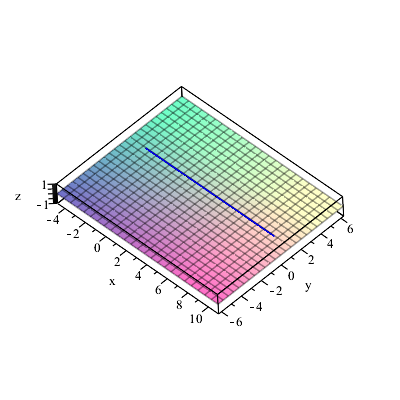
\includegraphics[width=\textwidth]{aeg0}
                \caption{\(a=0\). Længde af geodæt \(12,6\), længde af linje \(12,6\).}
                \label{fig:aeg0}
        \end{subfigure}%
        ~ %add desired spacing between images, e. g. ~, \quad, \qquad etc.
          %(or a blank line to force the subfigure onto a new line)
        \begin{subfigure}[b]{0.3\textwidth}
                \centering
                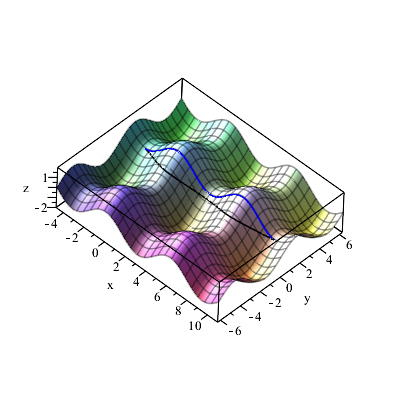
\includegraphics[width=\textwidth]{aeg1}
                \caption{\(a=1\). Længde af geodæt \(14,2\), længde af linje \(15,3\).}
                \label{fig:aeg1}
        \end{subfigure}
        ~ %add desired spacing between images, e. g. ~, \quad, \qquad etc.
          %(or a blank line to force the subfigure onto a new line)
        \begin{subfigure}[b]{0.3\textwidth}
                \centering
                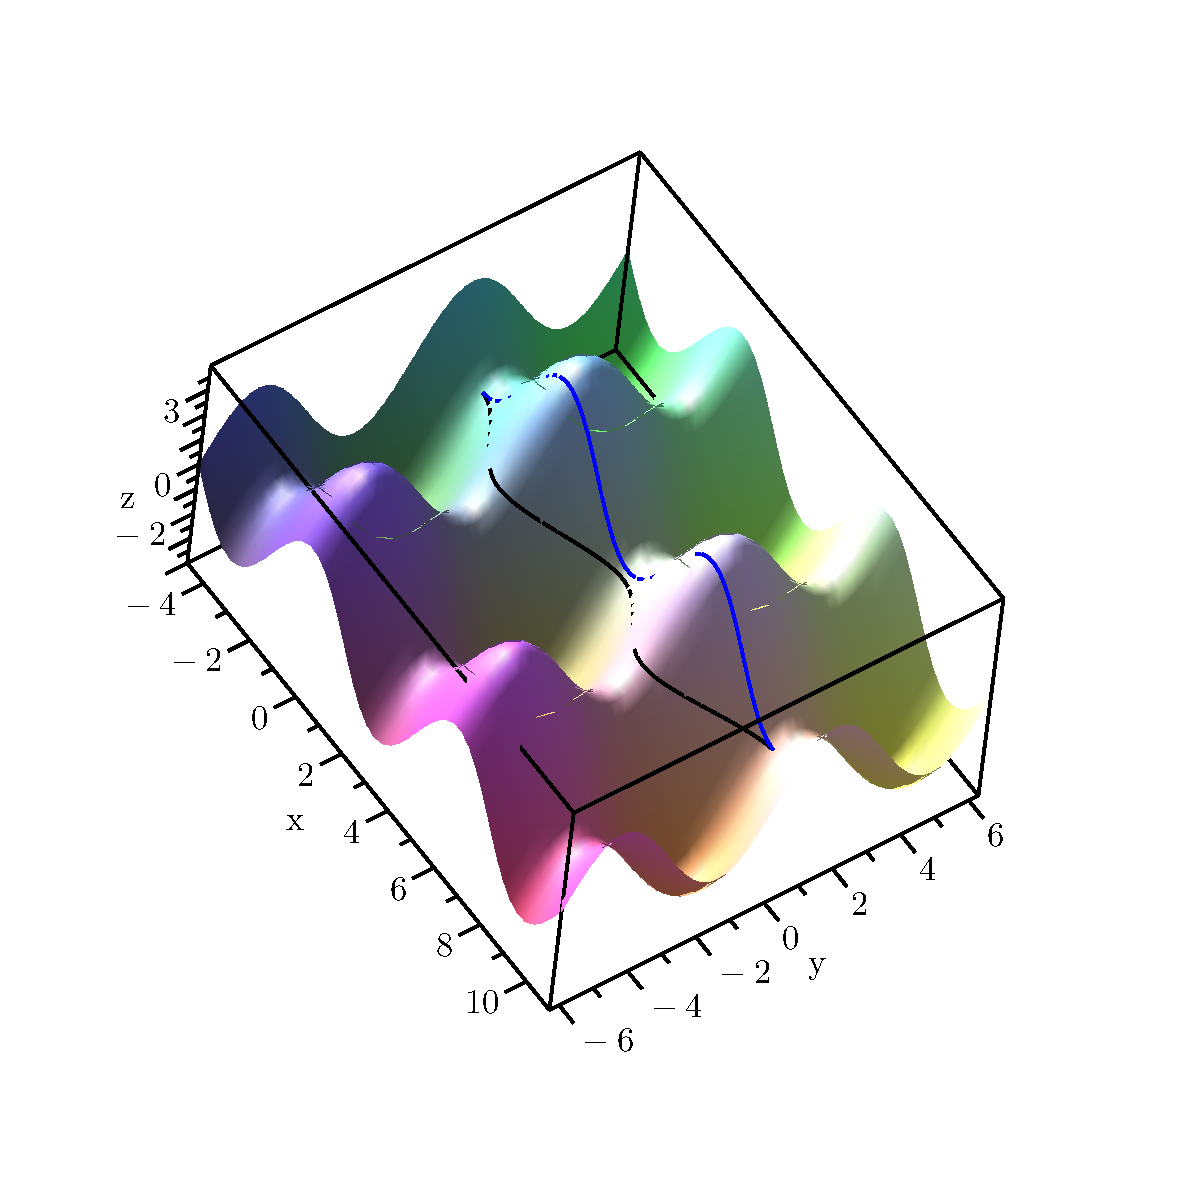
\includegraphics[width=\textwidth]{aeg2}
                \caption{\(a=2\). Længde af geodæt \(15,1\), længde af linje \(21,1\).}
                \label{fig:aeg2}
        \end{subfigure}
        \caption{
        Geodæter af typen \(\pmb{\gamma}(t) = (t,~m(t),~a\cos(t) + a\sin(m(t)))\) i sort;
        samt linjen (blå) der forbinder dennes endepunkter i \(\mathbb{R}^2\) projeceret på fladen \(F(x,~y)=(x,~y,~a\cos(x)+a\sin(y))\).}%\label{fig:animals}
\end{figure}

 \begin{figure}
        \centering
        \begin{subfigure}[b]{0.3\textwidth}
                \centering
                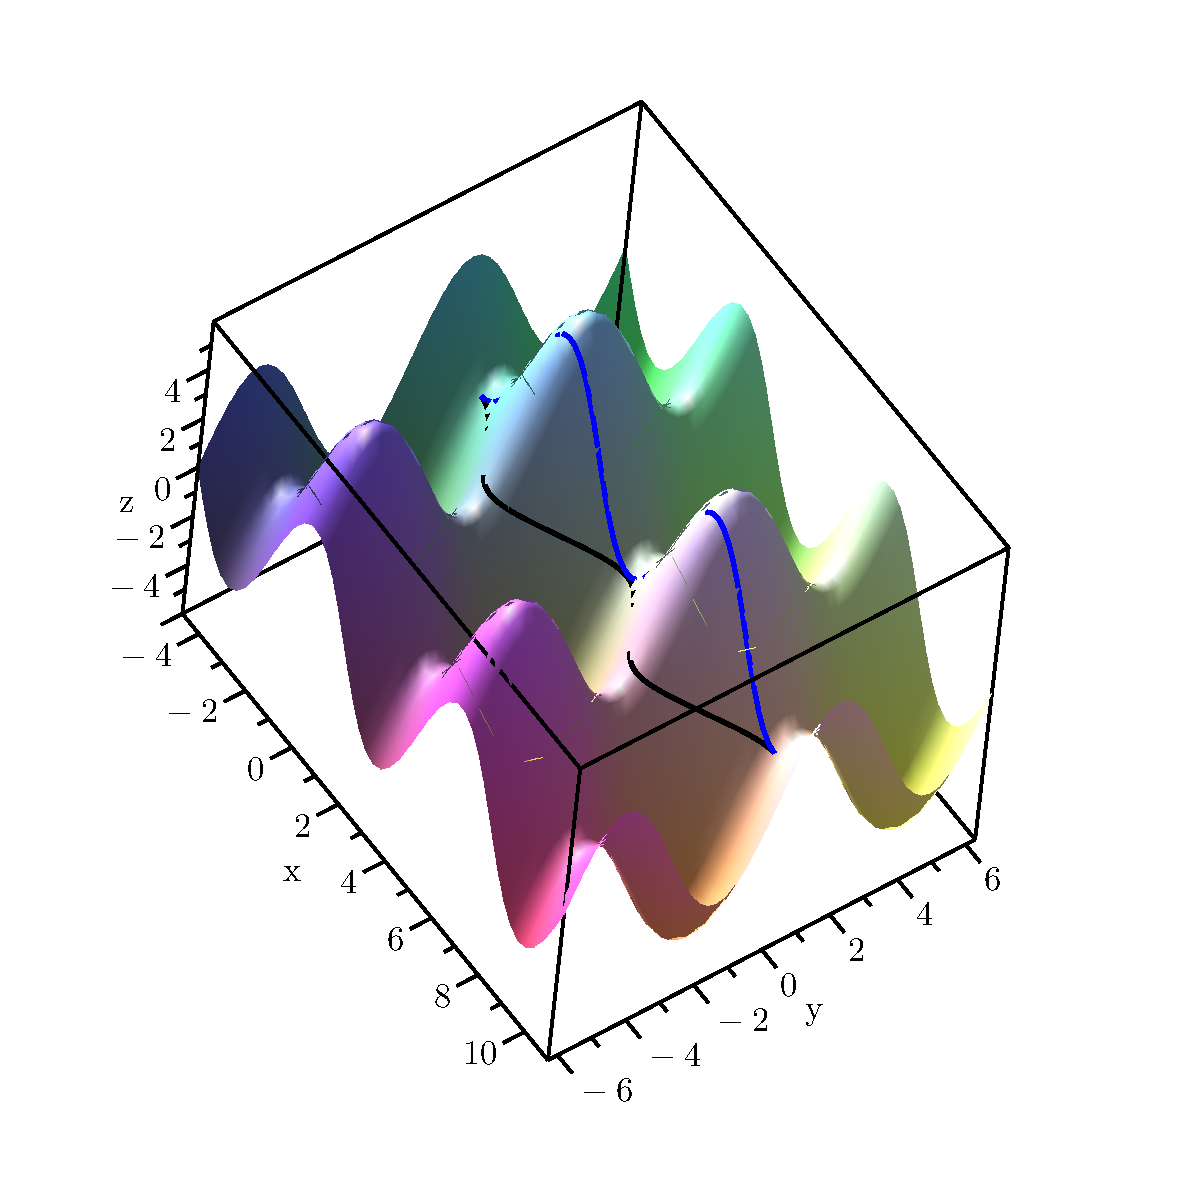
\includegraphics[width=\textwidth]{aeg3}
                \caption{\(a=0\). Længde af geodæt \(15,7\), længde af linje \(27,9\).}
                \label{fig:aeg3}
        \end{subfigure}%
        ~ %add desired spacing between images, e. g. ~, \quad, \qquad etc.
          %(or a blank line to force the subfigure onto a new line)
        \begin{subfigure}[b]{0.3\textwidth}
                \centering
                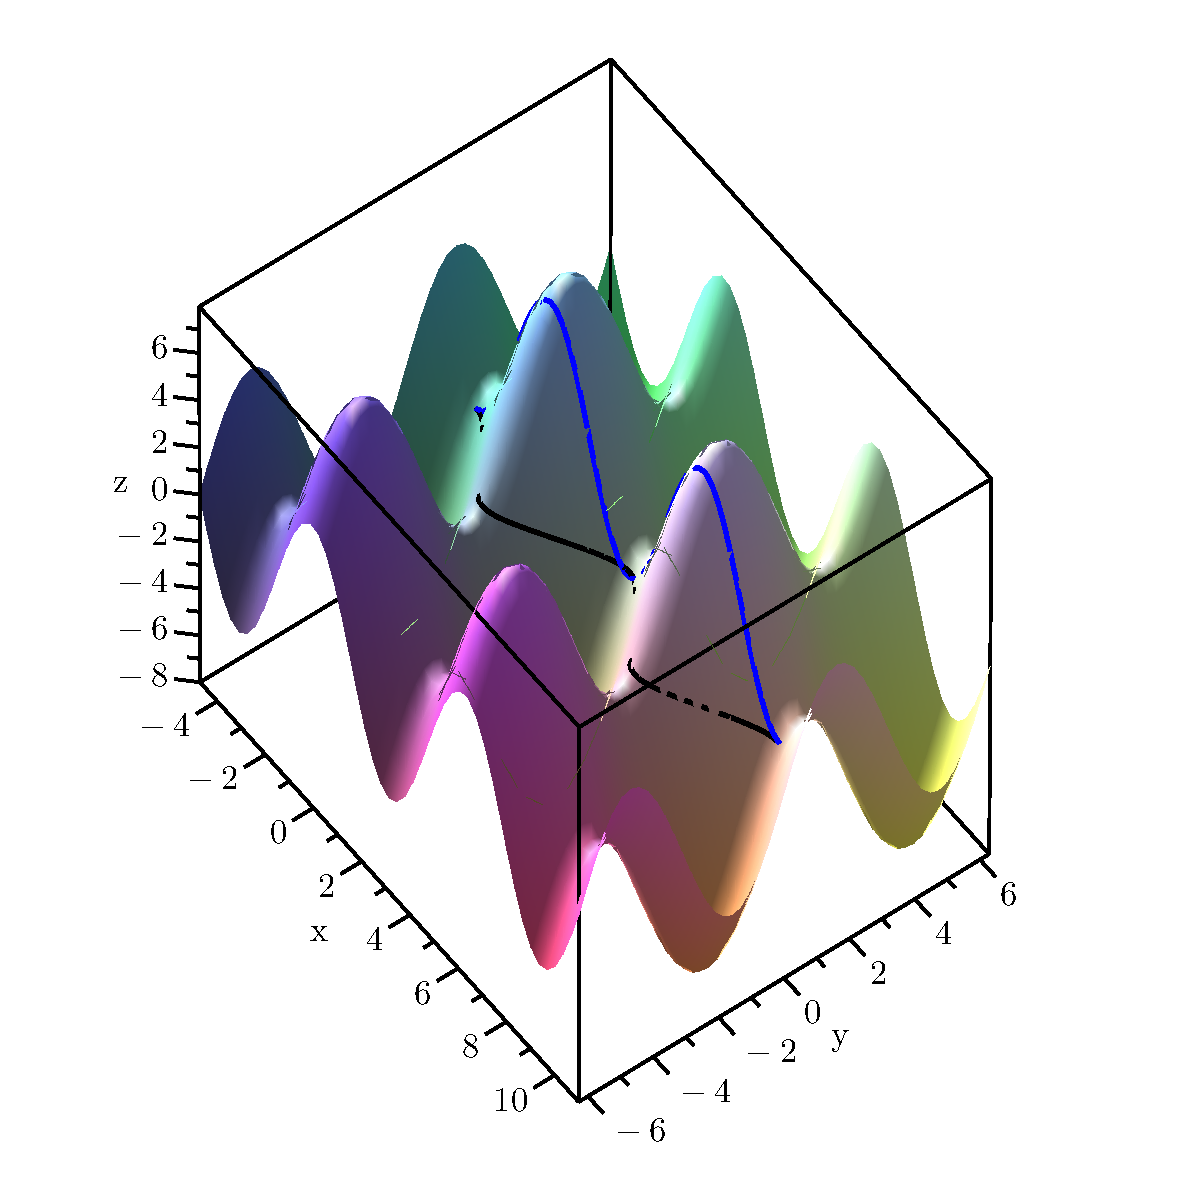
\includegraphics[width=\textwidth]{aeg4}
                \caption{\(a=4\). Længde af geodæt \(16,0\), længde af linje \(35,3\).}
                \label{fig:aeg4}
        \end{subfigure}
        ~ %add desired spacing between images, e. g. ~, \quad, \qquad etc.
          %(or a blank line to force the subfigure onto a new line)
        \begin{subfigure}[b]{0.3\textwidth}
                \centering
                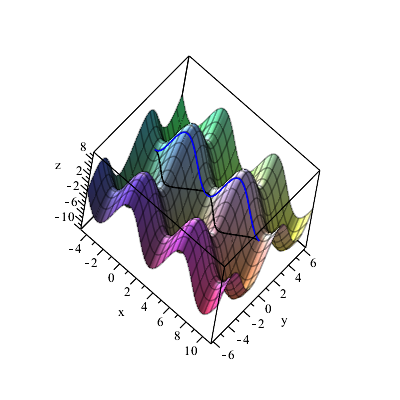
\includegraphics[width=\textwidth]{aeg5}
                \caption{\(a=5\). Længde af geodæt \(16,3\), længde af linje \(42,8\).}
                \label{fig:aeg5}
        \end{subfigure}
        \caption{
        Geodæter af typen \(\pmb{\gamma}(t) = (t,~m(t),~a\cos(t) + a\sin(m(t)))\) i sort;
        samt linjen (blå) der forbinder dennes endepunkter i \(\mathbb{R}^2\) projeceret på fladen \(F(x,~y)=(x,~y,~a\cos(x)+a\sin(y))\).}%\label{fig:animals}
\end{figure}

Det er dog langtfra alle geodæter, der kan findes med denne parametrisering. Der opstår tre problemer:
\begin{itemize}
\item To endepunkter vælges, der ikke giver en entydig geodæt (På æggebakken kan man eks. gå begge veje rundt om toppene)
\item Der findes løsninger til Euler-Lagrange ligningen, der ikke er geodæter. Eks er vejen lige over en top ikke altid den hurtigste vej,
men kan sagtens være den lokalt korteste.
\item Der kan findes geodæter, der ikke er af den type, parametriseringen dikterer.
\end{itemize}

De to første er primært et problem i forhold til den nummeriske løsning.
Endepunkter der resulterer i tvetydighed giver ofte enten fejl ved nummerisk løsning, eller en vej, der ikke er den korteste.
Derfor er endepunkterne i vores udregning valgt, som de er; da de ligger tilstrækkeligt langt fra problematiske punkter.

Desuden er der problemet i at der muligvis ingen geodæter findes for den givne parametrisering.
Så kunne man prøve sig frem med en anden parametrisering, men denne duer muligvis heller ikke.

Heldigvis findes der en anden måde til at finde geodæter nummerisk, dette vil næste afsnit behandle.

